\documentclass[conference]{IEEEtran}
\usepackage[T1]{fontenc}
\usepackage{microtype}
\usepackage{booktabs}
\usepackage{graphicx}
\usepackage{balance}
\usepackage{stfloats}
\usepackage[hidelinks]{hyperref}
\hypersetup{pdftitle={KVFold: Expanding Cache Capacity for LLM Agents with Lossless Compression},
            pdfsubject={ICDE demonstration paper}}
\title{KVFold: Expanding Cache Capacity for \mbox{LLM Agents} with Lossless Compression}
\author{\IEEEauthorblockN{Working draft}
\IEEEauthorblockA{Author information to be supplied}}
\raggedbottom
% Consistent space around floats; keep the IEEE text size and margins.
\setlength{\textfloatsep}{7pt plus 2pt minus 2pt}
\setlength{\dbltextfloatsep}{7pt plus 2pt minus 2pt}
\setlength{\intextsep}{7pt}
\begin{document}
\bstctlcite{kvfoldBibControl}
\maketitle

\begin{abstract}
Large language model (LLM) agents repeatedly reuse long prompt prefixes across
turns and resumed sessions, making key/value (KV) caching essential to avoid
redundant prefill computation. However, retaining these states in two-byte
bfloat16 (BF16) constrains serving at two levels: GPU memory bounds active
request concurrency, while external DRAM and NVMe capacity bounds how much
history survives before eviction forces recomputation. We present KVFold, a
lossless KV-cache compression system integrated with unmodified vLLM and
LMCache to turn saved bytes into usable capacity across GPU attention and
variable-length external storage. By preserving every BF16 low byte and
encoding frequent high bytes with calibrated short codes, KVFold expands
usable GPU KV capacity from 1.18M to 1.59M tokens on Qwen3-30B-A3B replays
under a 54~GB per-GPU budget. In the live demo, attendees edit and restore a
preset debugging prompt to inspect prefix reuse and check KV integrity after
re-import. Recorded coding-agent sessions then show how GPU capacity affects
queueing and how external cache capacity affects history retention.
\end{abstract}

\section{Introduction}
Key/value (KV) caching avoids repeated prefill computation by reusing attention
states across generation steps and shared-prefix requests. This reuse is
critical for LLM agents, whose multi-turn transcripts and subagent calls share
long contexts. Retaining these states, however, demands substantial capacity:
Qwen3-30B-A3B consumes 96~KB of bfloat16 (BF16) KV per token across all layers
(48~KB per rank at tensor-parallel degree~2). Consequently, capacity constrains
serving at two distinct levels---GPU KV memory bounds active concurrency,
whereas external DRAM and NVMe tiers govern how much history survives before
eviction forces costly recomputation.

Existing serving systems mitigate this overhead through sharing and offloading:
vLLM's PagedAttention~\cite{vllm} shares fixed-size blocks across requests,
while LMCache~\cite{lmcache} and Mooncake~\cite{mooncake} offload KV caches
across host DRAM and storage tiers. Yet every retained
BF16 value still occupies two bytes. While lossy quantization~\cite{kivi}
alters KV values and requires accuracy requalification, lossless compression
preserves exact values by exploiting recurring BF16 bit patterns; for example,
SplitZip~\cite{splitzip} codes frequent exponents for prefill-to-decode
transfer and reassembles original sign and fraction bits at the receiver.

Extending lossless compression from transfer to persistent prefix caches
introduces three systems constraints to convert saved bytes into effective
capacity. First, restoring to a contiguous buffer requires an extra scatter
pass into scattered GPU pages. Second, keeping GPU blocks compressed saves
memory only if attention decompresses them on the fly at native kernel speed.
Third, external tiers retain more history only when the allocator assigns exact
encoded lengths and keeps length readback off the load path.

Addressing these constraints, we present KVFold, a lossless KV-cache
compression system built on offline-calibrated per-head codebooks. Because BF16
low bytes carry near-full entropy (7.97 of 8 bits) while high bytes are
strongly skewed---the top seven values cover $\approx$94\% of occurrences in
Qwen3-30B-A3B (top 14 cover 99.81\%)---KVFold keeps low bytes verbatim and
codes high bytes with fixed-width two-level symbols across two modes:
\begin{itemize}
\item \emph{Pool mode} keeps completed blocks compressed inside shared-budget
GPU pages. Decode attention fuses register decompression with tensor-core
computation, and the worker exports the same records to LMCache unchanged.
\item \emph{Tier mode} retains unmodified native BF16 GPU pages and stock
attention kernels. LMCache stores exact-length compressed objects across DRAM
and NVMe and restores chunks directly into scattered GPU pages.
\end{itemize}

\section{KVFold Architecture}
\label{sec:design}
\subsection{Overview}
Figure~\ref{fig:architecture} illustrates KVFold across the GPU, PCIe, and
external cache tiers. Unmodified vLLM (v0.30) schedules requests and allocates
128-token logical blocks, while the LMCache server (v0.5.6) accesses engine
blocks over CUDA IPC and manages L1~DRAM and L2~NVMe lookup, LRU eviction,
write-through, and prefetch. In pool mode (Fig.~\ref{fig:architecture}a), an
out-of-tree attention plugin compresses closed blocks into the GPU pool and
exports immutable pool objects unchanged across PCIe. In tier mode
(Fig.~\ref{fig:architecture}b), vLLM runs stock FlashAttention-3
(FA3)~\cite{fa3neurips} on native BF16 pages while LMCache invokes KVFold's GPU
codec on saves and restores. Incompressible tier chunks cross PCIe as raw BF16.

\begin{figure*}[t]
\centering
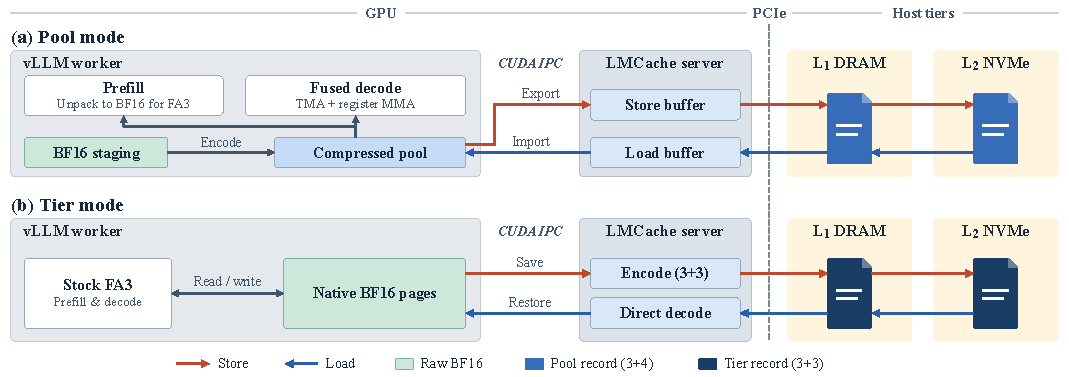
\includegraphics[width=0.96\textwidth]{images/KVFold_Fig1_Architecture.pdf}
\caption{KVFold integration across GPU memory, PCIe, and external cache tiers.
(a)~Pool mode stores compressed shared-budget pages on the GPU and exports them
unchanged to L1~DRAM and L2~NVMe. (b)~Tier mode retains native BF16 GPU pages
with stock FlashAttention-3 (FA3)~\cite{fa3neurips} and runs a server-side GPU
codec, transferring incompressible chunks as raw BF16.}
\label{fig:architecture}
\end{figure*}

\subsection{Lossless KV Encoding}
\label{sec:encoding}
Both modes store every BF16 low byte verbatim and encode the high byte (sign
plus upper seven exponent bits) using static offline-calibrated tables per
layer, KV head, and tensor (K or V). Inspired by lightweight database
compression---fixed-width codes with out-of-band exceptions~\cite{pfor,alp} and
lane-parallel layouts~\cite{fastlanes}---KVFold uses fixed-width symbols so
every warp lane reads at fixed offsets for lockstep parallel decoding. Each high byte first
receives a 3-bit primary code indexing the seven top entries in primary table
$P$, with \texttt{111} signaling an escape. The two modes specialize secondary
width and layout for their decoders: \emph{tier records} use a 3+3 code
(3-bit secondary indexing seven entries in extended table $E$, with
\texttt{111} escaping to an 8-bit raw byte) so all 14 entries fit in 16~B of
registers for branchless GPU \texttt{PRMT} lookup over token-ordered streams;
\emph{pool records} widen the secondary selector to 4~bits (3+4: 15 entries in
$E$, \texttt{1111} escaping to a 4~B raw patch), adding only 0.1\% to record
size while bounding per-warp raw patches so fused register decompression stays
loop-free.

\begin{figure}[!b]
\centering
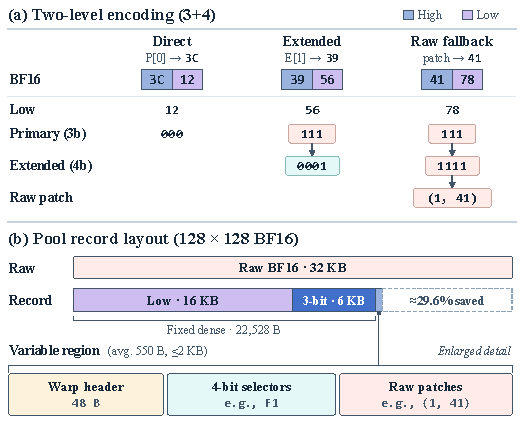
\includegraphics[width=0.97\columnwidth]{images/KVFold_Fig2_Encoding.pdf}
\caption{(a)~Two-level BF16 high-byte encoding in pool mode (3+4), where $P$
and $E$ are calibrated primary and extended tables (tier mode uses 3+3 for
register \texttt{PRMT} lookup). (b)~A 128-token pool record versus 32,768~B
of raw BF16. KB labels are approximate. The variable region is drawn at its
mean size (550~B, capped at 2,048~B) and enlarged below.}
\label{fig:record}
\end{figure}

The Direct, Extended, and Raw paths in Fig.~\ref{fig:record}a match the CPU
reference bit for bit on \texttt{3C12}, \texttt{3956}, and \texttt{4178}.
To test cross-domain reuse, we calibrated once per model on 1,024 agent tokens
(8.4~KB of tables for Qwen3-30B-A3B). Across seven domains, tier records
averaged 70.6\%--70.9\% of BF16 size on Qwen3-30B-A3B and GLM-4-9B-Chat-1M.
Per-domain calibration gained less than 0.1 percentage point.

\subsection{Pool Mode: GPU-Resident KV}
\label{sec:pool}
KVFold stages each active request's growing block in raw BF16 and encodes it
immediately after token~128 completes. Each pool record
stores one 128$\times$128 K or V tensor for one block, layer, and head
(32,768~B in BF16) in tensor-core MMA fragment order. The fixed dense part
occupies 22,528~B, with 16,384~B for low bytes and 6,144~B for 3-bit primary
codes. The variable region holds a 48~B warp header, 4-bit selectors, and
4~B raw patches. It averages 550~B and is capped at 2,048~B
(Fig.~\ref{fig:record}b). All $2H$ K/V records of a block and layer share one
compressed page with a pooled variable budget; at $H{=}4$, pages shrink from
256~KB to 186~KB (1.38$\times$ raw blocks before deducting staging, overflow,
record-map, and prefill buffers). Parallel encoders claim page space via an
atomic fill counter and publish \emph{(address, length)} in a per-layer record
map. Records whose variable region exceeds the cap or whose total size exceeds
the remaining page space fall back to 32,768~B raw overflow slots (0.03\% in
serving).

During \emph{prefill}, the plugin decodes cached pages into a BF16 workspace
for unmodified FA3 ($\le$3\% overhead). During \emph{decode}, a fused kernel
uses the Tensor Memory Accelerator (TMA) to prefetch records one step ahead
into dual shared-memory slots, decompresses each thread's 64 scalars directly
into registers without writing KV back to global memory, and executes
tensor-core MMAs with online softmax before merging partial states across page
ranges. Fixed padded-batch launch metadata preserves decode-only CUDA graph
replay. Although the fused kernel recovers the original BF16 KV bit for bit,
floating-point reduction order can cause its attention outputs to differ from
those of FA3.

For reuse after GPU eviction, the worker exports completed blocks with a
4~KB-aligned header. LMCache stores them unchanged. On a hit, the worker
imports them directly into GPU pages using atomic fill counters. If validation
fails, vLLM recomputes the block.

\subsection{Tier Mode: External KV Storage}
\label{sec:tier}
Tier mode keeps vLLM's native BF16 pages and stock FA3 on the GPU and compresses
chunks in LMCache. Each TP rank stores 128 tokens across all layers in one
record with a 4~KB header and padding to a 4~KB boundary for
\texttt{O\_DIRECT} NVMe I/O. Incompressible chunks stay raw. Within a
compressed record, KVFold splits each tensor into four streams (low bytes,
primary codes, secondary codes, and raw high bytes) and indexes 256-scalar
tiles in groups of eight (0.14 bits/scalar).

Three GPU kernels compress paged blocks without a gather pass. A background
worker waits on a CUDA event, reads encoded lengths in batches, allocates
exact-length L1~DRAM objects, and writes through to L2~NVMe. Loads never
wait for this \emph{deferred length readback}.
On loads, two CUDA streams rotate four buffers to overlap PCIe DMA with
multi-process GPU decompression. Warps use branchless \texttt{PRMT} lookup to
restore tiles directly into scattered GPU pages. Batches with raw chunks or
partially shared leading chunks use scratch space.

To measure scatter cost, we restored 256 chunks (3~GB of Qwen3-30B-A3B KV)
on one H800 SXM. SplitZip decoded at 1,215~GB/s into a contiguous buffer.
Including the scatter into GPU pages reduced throughput to 671~GB/s
(76.8\% of BF16 size). KVFold restored directly into GPU pages at
1,182~GB/s (70.9\%). In end-to-end tests, raw and tier modes produced
identical greedy output tokens on Qwen3-30B-A3B and GLM-4-9B.

% Declare Fig. 3 near the end of Section II so IEEEtran places it at the top of Page 3.
\begin{figure*}[!t]
\centering
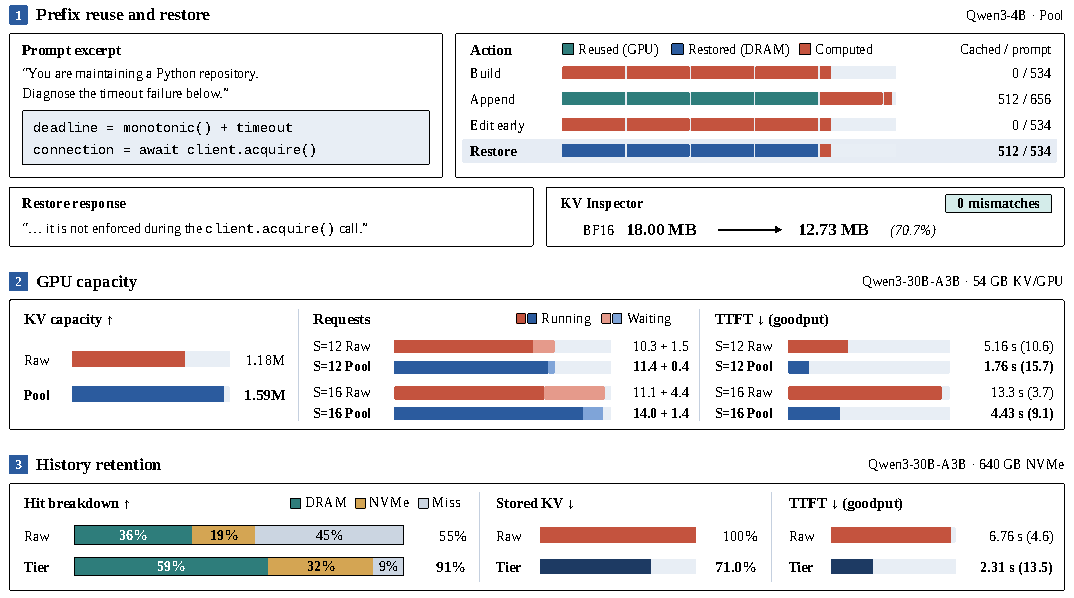
\includegraphics[width=0.94\textwidth]{images/fig3_console_update6.pdf}
\caption{Composite of selected views from the KVFold Console.
(1)~Live Qwen3-4B pool-mode interaction illustrating reused, restored, and
computed 128-token prefix blocks alongside the KV Inspector (18.00~MB BF16 to
12.73~MB encoded, zero export/import mismatches). (2)~Recorded AgentX GPU-capacity view
($P{=}64$, 54~GB KV/GPU, 400~GB DRAM, 2~TB NVMe): usable token capacity,
running vs.\ waiting requests in vLLM, and mean engine TTFT (with goodput in
req/min) at $S{=}12$ and $S{=}16$. (3)~Recorded AgentX history-retention view
($P{=}64$, $S{=}8$, 400~GB DRAM, 640~GB NVMe): prompt-token hit breakdown across
DRAM, NVMe, and misses, normalized stored KV size, and mean engine TTFT (with
goodput in req/min).}
\label{fig:views}
\end{figure*}

% Keep natural paragraph spacing below the full-width console figure.
\raggedbottom
\section{Demonstration Plan}
\label{sec:demo}
In the KVFold Console (Fig.~\ref{fig:views}, panel~1), attendees run four
live requests on a preset Python debugging prompt using Qwen3-4B in pool mode
(one H800 PCIe GPU, BF16 weights and KV). The recorded views relate GPU
capacity to request queues (panel~2) and external cache capacity to history
retention (panel~3). Both use Claude Code sessions from the InferenceX AgentX
benchmark~\cite{agentx} on Qwen3-30B-A3B (FP8 weights, BF16 KV, two H800
SXM GPUs, TP~2). Here $P$ counts live root sessions and a FIFO proxy admits
up to $S$ concurrent requests. For these runs, engine time to first token
(TTFT) excludes proxy wait. Goodput counts requests per minute with engine
TTFT $\le 2$~s and mean inter-token latency $\le 40$~ms.

\subsection*{Live Prefix Reuse and Restoration}
In the run shown in panel~1, \emph{Build} computes all 534 prompt tokens and
asynchronously exports completed 128-token blocks to LMCache DRAM in compressed
form. \emph{Append} adds the model's response and a preset test instruction.
The engine reuses 512 tokens (teal), recomputes the prompt's uncached 22-token
tail, and computes 122 new tokens. \emph{Edit early} changes
``Python'' to ``TypeScript'' within the first 128-token block. With no complete
prefix block to reuse, the engine recomputes all 534 tokens.
\emph{Restore} waits for pending external saves, flushes the GPU prefix cache,
and replays the original prompt. The engine restores 512 tokens directly
from LMCache DRAM into the compressed GPU pool (blue). The \emph{Build} and
\emph{Restore} responses both identify the missing timeout on
\texttt{client.acquire()}.

\emph{Build} also checks one completed 128-token block (36 layers, 576 records)
by exporting it through host memory and re-importing it into a separate GPU
scratch store. \mbox{The \emph{KV Inspector}}
shows its footprint (18.00~MB BF16, 12.73~MB encoded, 70.7\%). Attendees can
expand the Inspector to compare the SHA-256 digests of the BF16 values decoded
before export and after re-import. In this run, the digests match, and a
value-by-value comparison finds no differences across the 36 layers.

% Declare the paired tables on Page 3 so IEEEtran places them cleanly at the top of Page 4.
\begin{table*}[!t]
\begin{minipage}[b]{\columnwidth}
\centering
\caption{GPU capacity (54~GB KV/GPU, $P{=}64$, 400~GB DRAM, 2~TB NVMe,
0.94 hit share); Waiting and TTFT are means.}
\label{tab:gpu}
\small
\setlength{\tabcolsep}{3pt}
\begin{tabular*}{\columnwidth}{@{\extracolsep{\fill}}rlrrrr@{}}
\toprule
$S$ & Mode & KV tokens & Waiting &
\begin{tabular}[t]{@{}r@{}}TTFT\\(s)\end{tabular} &
\begin{tabular}[t]{@{}r@{}}Goodput\\(req/min)\end{tabular} \\
\midrule
12 & Raw  & 1.18M & 1.5 & 5.16 & 10.6 \\
12 & Pool & 1.59M & 0.4 & 1.76 & \textbf{15.7} \\
16 & Raw  & 1.18M & 4.4 & 13.3 & 3.7 \\
16 & Pool & 1.59M & 1.4 & 4.43 & \textbf{9.1} \\
\bottomrule
\end{tabular*}
\end{minipage}\hfill
\begin{minipage}[b]{\columnwidth}
\centering
\caption{History retention ($P{=}64$, $S{=}8$, 400~GB DRAM). Cached combines
DRAM and NVMe/GPU hit shares; TTFT is mean engine TTFT.}
\label{tab:tiers}
\small
\setlength{\tabcolsep}{3pt}
\begin{tabular*}{\columnwidth}{@{\extracolsep{\fill}}llrrr@{}}
\toprule
NVMe & Mode & Cached &
\begin{tabular}[t]{@{}r@{}}TTFT\\(s)\end{tabular} &
\begin{tabular}[t]{@{}r@{}}Goodput\\(req/min)\end{tabular} \\
\midrule
640~GB & Raw  & 0.55 & 6.76 & 4.6 \\
640~GB & Tier & 0.91 & 2.31 & \textbf{13.5} \\
2~TB   & Raw  & 0.94 & 1.69 & 15.1 \\
2~TB   & Tier & 0.94 & 1.73 & 15.1 \\
\bottomrule
\end{tabular*}
\end{minipage}
\end{table*}

\subsection*{GPU Capacity under Concurrent Load}
The recorded views show how serving metrics guide mode selection. When
external tiers already retain the active working set (0.94 cached-token share
at 400~GB DRAM and 2~TB NVMe), rising concurrency makes GPU KV capacity the
primary bottleneck. Under a 54~GB per-GPU KV budget, pool mode holds 1.59M
usable tokens (1.34$\times$ raw's 1.18M) after reserving 1.3~GB inside the
budget for staging, overflow, record maps, and prefill workspace; cache-server
CUDA contexts and transfer buffers lie outside this budget.

At the low-load baseline ($S{=}8$), both modes show little queueing, with
goodput of 15.1~req/min in raw mode and 16.3 in pool mode. To see how the two
modes respond as queues form, attendees compare the higher-load runs at
$S{=}12$ and $S{=}16$ shown in Fig.~\ref{fig:views} (panel~2) and
Table~\ref{tab:gpu}.
At $S{=}12$, raw mode averages 1.5 waiting requests and its mean engine TTFT
rises to 5.16~s. Pool mode averages 0.4 waiting requests, cuts mean engine
TTFT to 1.76~s, and raises goodput from 10.6 to 15.7~req/min, just above
raw mode at $S{=}8$ with a 50\% higher concurrency limit.
At $S{=}16$, pool mode sustains 14.0 running requests
on average (vs.\ 11.1 in raw mode) and delivers 2.5$\times$ the goodput
(9.1 vs.\ 3.7~req/min).

\balance
\subsection*{History Retention under Storage Pressure}
When high miss rates or heavy NVMe traffic indicate external tier exhaustion,
attendees switch to the history-retention view (Fig.~\ref{fig:views}, panel~3;
Table~\ref{tab:tiers})
and compare two NVMe budgets at $S{=}8$. Raw and tier modes both use native
GPU pages, stock FA3, and the same LMCache LRU, write-through, and prefetch
policies. Tier mode's store and rotating load buffers occupy
approximately 2.5~GB per GPU outside the KV budget.

At 640~GB NVMe, raw LMCache falls off its LRU eviction cliff: cached-token
share collapses to 0.55 (36\% DRAM, 19\% NVMe, 45\% recomputed misses), pushing
mean engine TTFT to 6.76~s and goodput down to 4.6~req/min. Compressing stored
KV to 71.0\% of raw bytes makes the tiers behave like 1.4$\times$ larger raw
tiers---lifting total cached share to 0.91 while promoting hits from NVMe into
DRAM (59\% DRAM, 32\% NVMe, 9\% misses). Tier mode thus cuts mean engine TTFT
by 2.9$\times$ (2.31~s) and raises goodput by 2.9$\times$ (13.5~req/min). At
2~TB NVMe, where raw capacity already holds the working set (0.94 hit share),
compression adds minimal overhead: goodput matches raw (15.1~req/min), mean
engine TTFT stays within 0.04~s (1.73 vs.\ 1.69~s), and prompt throughput drops
by only 2.2\% (26.9 vs.\ 27.5 thousand tokens/s).

Across the two recorded comparisons, pool mode shortens queues when GPU KV
capacity limits concurrency, while tier mode reduces recomputation when the
external cache is too small to retain the working set.

\section*{Acknowledgment}
% Replace the reserved space below with two or three lines of acknowledgments.
\par\vspace*{3\baselineskip}

\bibliographystyle{IEEEtran}
\bibliography{references}
\end{document}
